
% Inbuilt themes in beamer
\documentclass[aspectratio=169]{beamer}
\usepackage{graphicx}
% Theme choice:
\usetheme{CambridgeUS}

% Title page details: 
\title{Econometrics Discussion Section 2} 
\author{John Green}
\date{Spring 2024}


\begin{document}

% Title page
\begin{frame}
    \titlepage 
\end{frame}

% Outline frame
\begin{frame}{Omitted Variable Bias}
    \begin{itemize}
        \item In economics, we often want to determine the impact of $X$ on $Y$
        \begin{itemize}
            \item But $X$ is not the only thing going on! Usually many variables are effecting $Y$
            \item If we don't include these other variables in our model, we will get biased estimates of the effect of $X$ on $Y$, a problem referred to as \textit{omitted variable bias}
        \end{itemize}
        \item Let's think about what this does to our estimate with a silly example
        \begin{itemize}
            \item We are an AC company, and we want to know what causes people to buy more AC units
            \item Our statistician tells us that the number of swimming pool accidents is a good predictor of AC units sold
            \item We run a regression of AC units sold on swimming pool accidents and find a positive relationship
            \item Should we conclude that swimming pool accidents cause people to buy more AC units?
        \end{itemize} 
    \end{itemize}
\end{frame}

\begin{frame}{Omitted Variable Bias}
    \begin{itemize}
        \item Should we conclude that swimming pool accidents cause people to buy more AC units?
        \item Of course not! The omitted variable here is temperature. When it's hot, people buy more AC units and more people go swimming
        \item Intuitively, what direction do we expect the bias in the effect of swimming pool accidents to be?
    \end{itemize}
\end{frame}

\begin{frame}{Omitted Variable Bias}
    \begin{itemize}
        \item Should we conclude that swimming pool accidents cause people to buy more AC units?
        \item Of course not! The omitted variable here is temperature. When it's hot, people buy more AC units and more people go swimming
        \item Intuitively, what direction do we expect the bias in the effect of swimming pool accidents to be?
        \item It should bias the estimate \textit{upwards}: we are attributing the effect of temperature to swimming pool accidents and thus making swimming pool accidents look more important than they are
    \end{itemize}
\end{frame}

\begin{frame}{Omitted Variable Bias}
    \begin{itemize}
        \item We have omitted variable bias when we have a variable $Z$ that is correlated with $X$ and is a determinant of $Y$
        \begin{itemize}
            \item Note: if $Z$ is a determinant of $Y$ but is not correlated with $X$, then it is not a problem!
            \item These conditions mean that our OLS assumption of $E(u|X) = 0$ is violated
        \end{itemize}
        \item Formula for OVB:
        $$
        \hat{\beta} \to_{p} \beta + \frac{\sigma_u}{\sigma_X}\rho_{Xu}
        $$
        \begin{itemize}
            \item The intuition from our example shows up in the correlation term
        \end{itemize}
    \end{itemize}
\end{frame}

\begin{frame}{Causal effects}
    \begin{itemize}
        \item We can use OLS to summarize a relationship without attaching any directionality
        \begin{itemize}
            \item In this case we need to be careful in our language: "a change in X is associated with a change in Y"
        \end{itemize}
        \item Usually economists want to be able to say something \textit{causal}
        \item Ideal is a randomized controlled trial (RCT): some group gets the treatment, some group doesn't, and we compare outcomes between the two
        \begin{itemize}
            \item Observational data usually differs from this in important ways
        \end{itemize}
    \end{itemize}
\end{frame}

\begin{frame}{Solution to OVB}
    \begin{itemize}
        \item An RCT eliminates OVB because we randomly assign the treatment, which will then not be correlated with any other variables!
        \begin{itemize}
            \item This is usually not possible in economics --- this is why economics is hard!
        \end{itemize}
        \item Cross-tabulation eg run the regression on a subsample of your population where there is no OVB problem (but other issues emerge)
        \item Try and include omitted variables (obviously) in a multivariable regression
    \end{itemize}
\end{frame}

\begin{frame}{Multivariate regression}
    \begin{itemize}
        \item Same logic as before:
        $$
        Y_i = \beta_0 + \beta_1X_{1i} + \beta_2X_{2i} + u_i    
        $$
        \item Estimators derived in same way as before (just using matrices)
        \item Before we looked at $R^2$ as a measure of fit, but now we have to be careful: adding in more variables on the RHS will always increase $R^2$
        \item Adjusted $R^2$ is a better measure of fit which includes a degrees-of-freedom correction to penalize for adding in more variables
        \item Add one more assumption our previous 3 from the single-variable case: no perfect multicolinearity
    \end{itemize}
\end{frame}

\begin{frame}{Perfect multicolinearity}
    \begin{itemize}
        \item This is when one of your RHS variables is a perfect linear combination of others
        \item Why is this a problem?
    \end{itemize}
\end{frame}

\begin{frame}{Perfect multicolinearity}
    \begin{itemize}
        \item This is when one of your RHS variables is a perfect linear combination of others
        \item Why is this a problem?
        \item Think about basic algebra:
        \begin{itemize}
            \item $y = a*x$
            \item What is $a$?
        \end{itemize}
    \end{itemize}
\end{frame}

\begin{frame}{Perfect multicolinearity}
    \begin{itemize}
        \item $y = a*x$
        \item What is $a$?
        \item $a = \frac{y}{x}$
        \item But now what if I give you:
        \begin{itemize}
            \item $y = b*x + c*x $
            \item What are $a$ and $b$?
        \end{itemize}
    \end{itemize}
\end{frame}

\begin{frame}{Perfect multicolinearity}
    \begin{itemize}
        \item But now what if I give you:
        \begin{itemize}
            \item $y = b*x + c*x $
            \item What are $b$ and $c$?
        \end{itemize}
        \item This question has no unique answer! Any combination of $b$ and $c$ such that $a = b + c$ will work (an infinite number)
        \item This is what's going on when their is perfect multicolinarity: our coefficient estimates $\beta$ are not identified/unique
    \end{itemize}
\end{frame}

\begin{frame}{Binary variables}
    \begin{itemize}
        \item For this reason we need to be careful when we have binary (0/1) variables (``indicator'' variables) in our regression:
        \begin{itemize}
            \item Treatment status
            \item Gender
            \item Party affiliation
        \end{itemize}
        \item We either need to leave one out (the omitted group) or we need to drop our intercept
        \begin{itemize}
            \item Either is fine, just changes interpretation of the coefficient estimates
            \item Failing to do so is sometimes called the the ``dummy variable trap''
        \end{itemize}

        \pause

        \item Exact same math, intuition, problem and solution extends to \textit{categorical} variables:
        \begin{itemize}
            \item Seasonal effects
            \item Race or ethnicity
        \end{itemize}
        \item In practice, we take our categories and create a bunch of dummy variables, so we need to leave one category out as the ``base'' to avoid multicolinearity
    \end{itemize}
\end{frame}

\begin{frame}{Imperfect multicolinearity}
    \begin{itemize}
        \item Perfect multicolinearity is straightforward to deal with; generally speaking, the regression simply will not work
        \item Slightly trickier is \textit{imperfect} multicolinearity: $X_1$ and $X_2$ are highly correlated
        \begin{itemize}
            \item For example, controlling for both age and years of work experience in a wage equation
        \end{itemize}
        \item Imperfect multicolinearity will lead to imprecise estimation (large standard errors)
        \item Intuition: what does the data tell us about the effect of $X_1$ when $X_2$ is held constant?
        
        \pause

        \item What can we do?

        \pause

        \item Can check scatterplots: if two variables are essentially linear together, probably only include one of them
        \item Guided by theory: it's usually obvious if two variables are highly linear
    \end{itemize}
\end{frame}

\begin{frame}{Control variables}
    \begin{itemize}
        \item Usually, we cannot just include the omitted variables
        \item Instead, look for control variable(s) $W$ which are correlated with the omitted variables
        \item Helps us address the OVB problem and get the causal impact of a variable X ($\to$ conditional mean independence holds)
        \item Example: impact of years of higher education on wages
        \begin{itemize}
            \item Problem: ability is correlated with both! (In which direction is OVB?)
            \item Solution: control for ability, eg use parental income, quality of local high schools, etc.
        \end{itemize}
    \end{itemize}
\end{frame}

\begin{frame}{Residuals}
    \begin{itemize}
        \item Usually, we cannot just include the omitted variables
        \item Instead, look for control variable(s) $W$ which are correlated with the omitted variables
        \item Helps us address the OVB problem and get the causal impact of a variable X ($\to$ conditional mean independence holds)
        \item Example: relationship between GPA and job performance
        \begin{itemize}
            \item Problem: ability is correlated with both! (In which direction is OVB?)
            \item Solution: control for ability, eg use parental income, quality of local high schools, etc.
        \end{itemize}
    \end{itemize}
\end{frame}

\begin{frame}
    \centering
    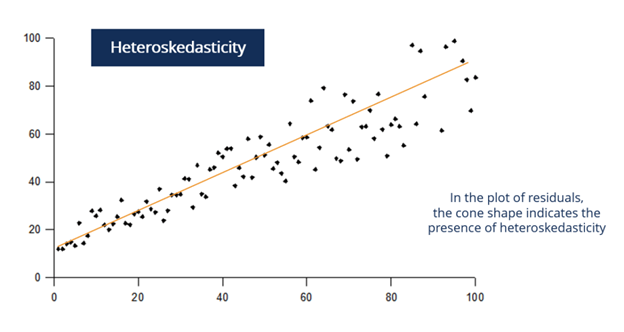
\includegraphics[width = .75\textwidth,keepaspectratio]{./figs/heteroskedasticity.png}
\end{frame}

\begin{frame}{Hypothesis testing}
    \begin{itemize}
        \item We already know about the hypothesis test on a single coefficient: simple t-test with a known distribution
        \item What about a joint hypothesis test? For example:
        \begin{itemize}
            \item $H_0:~\beta_1 = \beta_2 = 0$
            \item $H_0:~\beta_1 = \alpha_1~\&~\beta_2 = \alpha_2$
        \end{itemize}
        \item What is the difference between testing this hypothesis one piece at a time, and testing them together (a \textit{joint} test)?
        \item What is the alternate hypothesis?

        \pause
        \item $H_A: \beta_1 \neq \alpha_1~ \text{or} ~\beta_2 \neq \alpha_2)$
        \item These two events will not be independent: so $P(\beta_1 \neq \alpha_1~ \text{or} ~\beta_2 \neq \alpha_2) $ cannot be derived just by considering the probabilities each on their own with a t-test
    \end{itemize}
\end{frame}

\begin{frame}{Joint hypothesis test}
    \begin{itemize}
        \item To test a joint hypothesis, we can use an $F$-statistic which follows a $\chi^2_q$ distribution where $q$ is degrees of freedom
        \item Intuition: look at the fit of the regression under the null and alternate hypotheses; if fit under the null is much worse than under the alternate, reject the null
        \begin{itemize}
            \item What do we use to check for fit?
            \pause
            \item Test statistic based on $R^2$
        \end{itemize}
        \item Just like the Normal distribution is defined by a mean and variance, $\chi^2_q$ is defined by \textit{degrees of freedom}
        \item In this case, Degrees of freedom is our number of restrictions
        \begin{itemize}
            \item Under the hood: this is the number of squared normal random variables in the test statistic
            \item What might happen as we add in more restrictions?
        \end{itemize}
    \end{itemize}
\end{frame}

\begin{frame}{F-test}
    \begin{itemize}
        \item This F-test is very powerful:
        \item Can test complex hypotheses over multiple coefficients
        \item Confidence \textit{set} for coefficients: all combos not rejected under a given test 
        \item In practice: most common F-test is that ``our data matters''
        \begin{itemize}
            \item $Y = \beta_0 + \beta_1 X_1 + \beta_2 X_2 + \epsilon $
            \item F-test for $\beta_1 = \beta_2 = 0 $
            \item E.g., do we do meaningfully better at explaining variation in $Y$ with our $X$ variables than we would by just taking the mean?
            \item This F-stat automatically reported in stata
        \end{itemize}
    \end{itemize}
\end{frame}

\begin{frame}{Hypotheses on coefficient relationships}
    \begin{itemize}
        \item Sometimes we may have a hypothesis on how $\beta_1$ and $\beta_2$ relate to each other, but not on their specific values
        \item Eg $\beta_1 = \beta_2 $ in $Y = \beta_0 + \beta_1 X_1 + \beta_2 X_2 + \epsilon $
        \item Often, we can use simple algebra to rewrite our model in a way that is easy to test:
        \begin{equation*}
            \begin{split}
                Y &= \beta_0 + \beta_1 X_1 + \beta_2 X_2 \\
                &= \beta_0 + \beta_1 X_1 + \beta_1 X_2 \\
                &= \beta_0 + \beta_1 \left( X_1 + X_2 \right) \\
                &= \beta_0 + \beta_1 \left( X_{12} \right)
            \end{split}
        \end{equation*}
        \item So, just make a new variable $X_{12}$ and do an F-test for the restricted regression against the unrestricted regression
    \end{itemize}
\end{frame}

\begin{frame}{Hypotheses on coefficient relationships}
    \begin{itemize}
        \item Might get more complicated, with more coefficients and different relationships
        \item Math (and code) becomes easier if we can write our restrictions in the form:
        $$
        a_1 \beta_1 + a_2 \beta_2 + \dots + a_k \beta_k = 0
        $$
        \item Our example is $Y = \beta_0 + \beta_1 X_1 + \beta_2 X_2 + \epsilon $ and $ H_0: ~ \beta_1 = \beta_2$
        \begin{itemize}
            \item Want to write in the form $a_1 \beta_1 + a_2 \beta_2 = 0$
            \item What are $a_1$ and $a_2$?
            \pause
            \item $ \beta_1 = \beta_2 \rightarrow \beta_1 - \beta_2 = 0$ so $a_1 = 1$ and $a_2 = -1$
        \end{itemize}
    \end{itemize}
\end{frame}


\end{document}